%!TEX root = ../article.tex

% Conclusion
\section{Fazit}
\label{sec:fazit}
Die gezeigte Methode ermöglicht unterschiedlich große und komplexe Oberflächen über den Marching Cubes Algorithmus zu rendern, die aus einer konstruierten Voxelstruktur mit dynamischen Füllmengen und unterschiedlichen Materialien bestehen. Dabei werden sämtliche gestellte Anforderungen erfüllt.

\begin{figure}[H]
			\centering
			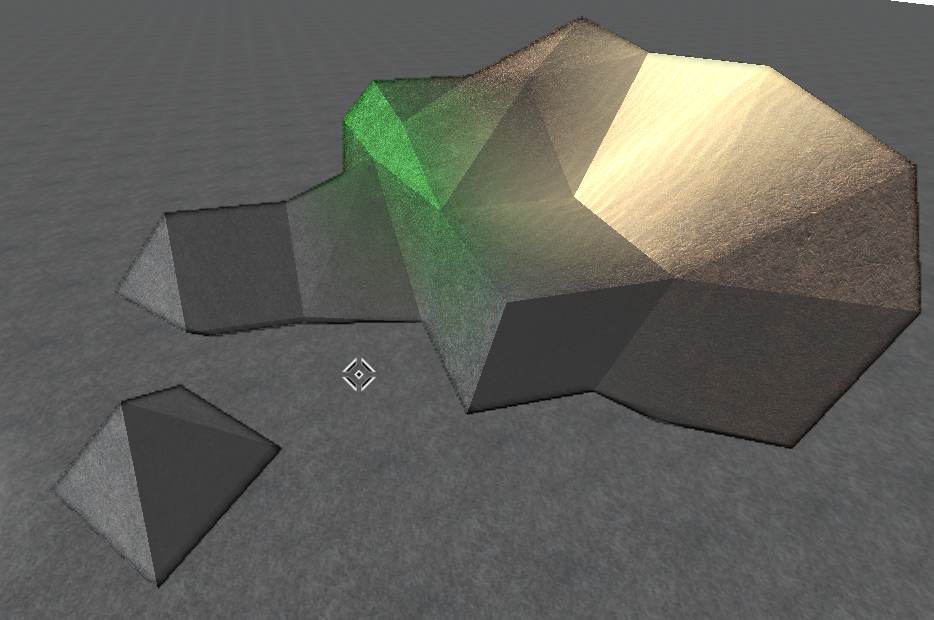
\includegraphics[width=0.5\textwidth]{figures/ProjectImage}
			\caption[Beispiel aus dem Projekt\cite{project}]{Beispiel aus dem Projekt \label{MarchingCubesPossibilities}}
\end{figure}